\section{Sistema A + C}


Para junção dos sistemas A e C em termos de código foi apenas utilizado multitasking por timer para poder fazer correr as funções de ambos os sistemas em sincronia. Foi ainda adicionado um sensor ultrassónico para poder fazer a paragem do servomotor.

\begin{figure}[H]
    \centering
    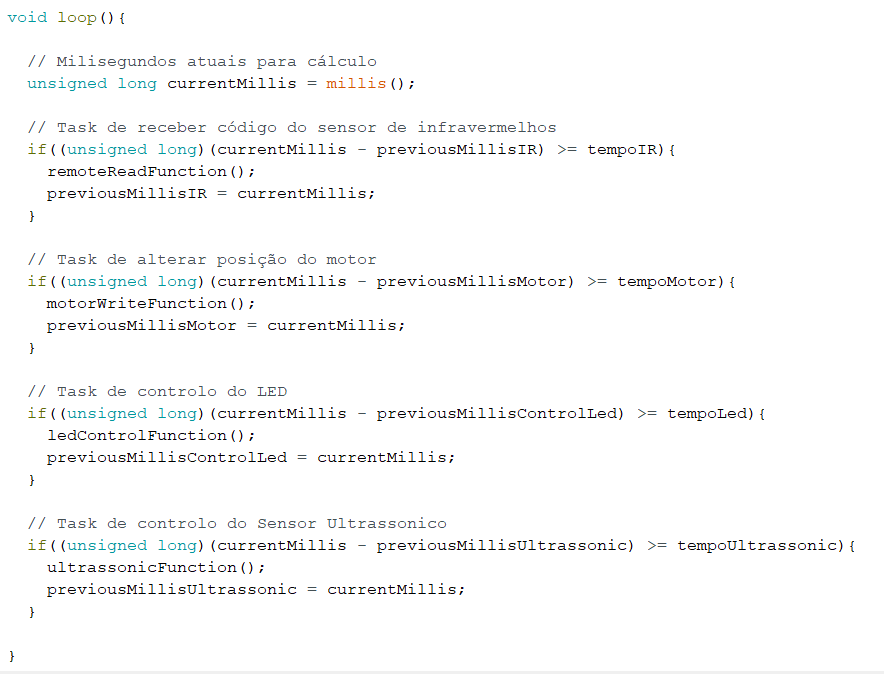
\includegraphics[scale=0.45]{images/codigo/sisACMultitasking.png}
    \selectlanguage{portuguese}\caption{Loop Multitasking}
\end{figure}


\begin{figure}[H]
    \centering
    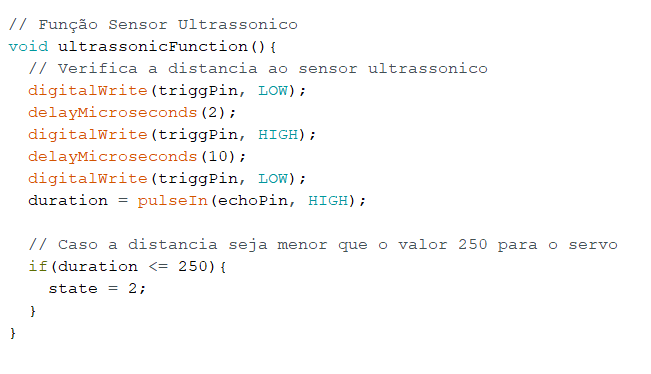
\includegraphics[scale=0.45]{images/codigo/sisAC_ultra.png}
    \selectlanguage{portuguese}\caption{Função Sensor Ultrassónico}
\end{figure}

